\documentclass[preprint,natbib,10pt]{article}

%\usepackage[left=2cm,top=1cm,right=3cm,nohead,nofoot]{geometry}
\usepackage[left=3cm,top=1cm,right=3cm]{geometry}

% the algorithm2e package
\makeatletter
\newif\if@restonecol
\makeatother
\let\algorithm\relax
\let\endalgorithm\relax
%%\usepackage[figure,ruled,vlined]{algorithm2e}
\usepackage[ruled,vlined]{algorithm2e}

\usepackage{amsmath}
\usepackage{listings}

\usepackage{graphicx}
\DeclareGraphicsRule{.jpg}{eps}{.bb}{}
\DeclareGraphicsRule{.png}{eps}{.bb}{}
\graphicspath{{./} {figures/}}

% Setup TikZ
\usepackage{tikz}
\usetikzlibrary{shapes} % ecllipse
\usetikzlibrary{arrows}
\tikzstyle{block}=[draw opacity=0.7,line width=1.4cm]

\begin{document}
\renewcommand\figurename{Figure}

% define the title
\title{The Algorithms Used in the Supertile Simulation System (Draft)}
\author{Yunhui Fu}
\date{} % <--- leave date empty

% \authorinfo{Yunhui Fu}
%            {Computer Science Department, Texas University-Pan American, Edinburg TX, USA}
%            {yfu@broncs.utpa.edu}

%generates the title
\maketitle

%insert the table of contents
\tableofcontents

\section{Introduction}
Tiles are some squares with four glues at each of the sides. Supertiles are the complex structure composed by some tiles. The tiles have to combine with each other in each edge with the dovetailed glue. All of the tiles and supertiles are two-dimension.

The X-Y coordinate system we used in this paper is defined by comparing the sequence of the array structure of C language. The items of the array are placed in the memory one by one, left to right and up to down. The positive orientation of the Y axis is from bottom to up; the positive orientation of the X axis is from left to right. The start value of the axis is 0. There are some examples of the coordinates: (0,0), (0,1), (1,0), (0, 2).

To simulate the supertile system, we use a array which records all types of the supertiles created during the simulation and it's quantity. In each loop, two types of supertile(can be the same type) is pick out randomly to test if them could mesh with each other. If the two supertiles could mesh with each other, the new supertile will be stored in the array.

\section{The Main Algorithms}
Two tests are important in this simulation system. One is Equivalence Testing, another one is Mesh Testing.

\begin{enumerate}
  \item Equivalence Testing (ET)

Equivalence Testing is used to test if two supetile is equal. The supertiles are placed at random orientation. The supertile have to rotate at most four times and compare with another supertile to see if the two supertils are equal. 

This type of testing is used in the statistic of the numbers of created supertiles.

  \item Mesh Testing (MT)

To test if two supertile could be engaged with each other at a given tempreture. We should consider the condition that one supertile should not enter the hollow in the center of other supertile. (If this type of testing will consume much of the time, we can consider to cache the result, such as store it to database, such as sqlite.)

Let's say that one of supertile is named Base which is tested, another one is named Test.
The orientation of one supertile is the rotate times of the supertile from the origin state in the list table. Each of the rotate angle is $0^{\circ}, 90^{\circ}, 180^{\circ}$, and $270^{\circ}$. After each rotate, the Test supertile will try to mesh with the Base supertile. Thus the Test supertile have to rotate four times to mesh with the Base supertile.

 Let's say that the testing at the edge is named Sliding Testing(ST). There will be four times Sliding Testing for each orientation of Test supertile. The begin position for the Test supertile to test if it can mesh with the Base supertile have to be at the outer side of the Base edge because of the geometry shape. For each of the Sliding Testing, the Test supertile is placed at the edge of the Base supertile, with only one point of the area adjoin with. Then it will be tested for meshing with Base, which is called Plumb Testing(PT). After one Plumb Testing, the Test supertile will move to the next point of the same direction of Sliding Testing.

Say that MaxTestX is the maximum length of Test, and MaxTestY is the maximum width of Test; MaxBaseX is the maximum length of the Base, and MaxBaseY is the maximum width of the Base. As the figure show, Base is fixed at the position (MaxTestX, MaxTestY).

There will be two start positions for the Test to start Sliding Testing, the position (0,0) and (MaxTestX + MaxBaseX, MaxTestY + MaxBaseY). The Test will test four times of the sliding testing. The Test will slide to two directions for each position; The sliding testing will also try the positions at the plumb of the direction of sliding.

\begin{figure}\centering
  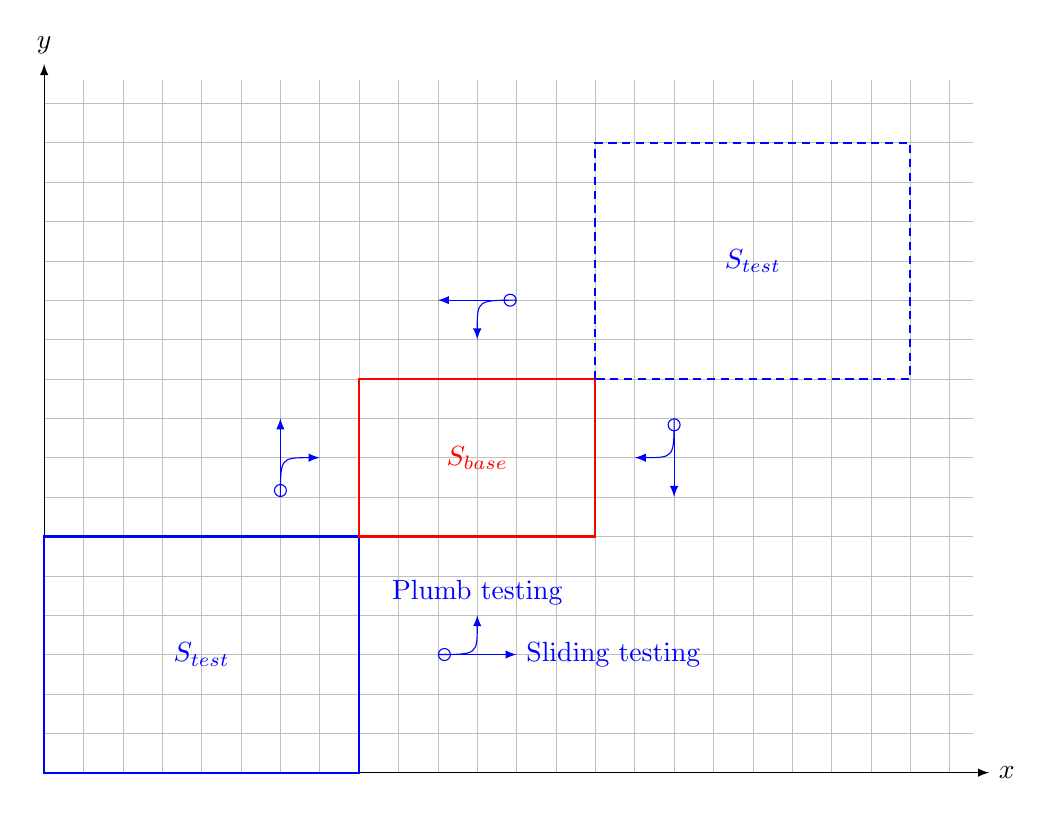
\begin{tikzpicture}
    \draw[step=.5cm,gray!50!white,very thin] (0,0) grid (11.8, 8.8);%(5.8,4.3);
    \draw[-latex] (0,0) -- (12,0) node [anchor=west] {$x$};
    \draw[-latex] (0,0) -- (0,9) node [anchor=south] {$y$};

    \draw[blue,thick] (0,0) rectangle (4,3) (2,1.5) node {$S_{test}$};
    \draw[red,thick] (4,3) rectangle (7,5) (5.5,4) node {$S_{base}$};
    \draw[blue,thick,densely dashed] (7,5) rectangle (11,8) (9,6.5) node {$S_{test}$};

    \draw[o-latex,blue] (6,6) -- (5,6);
    \draw[-latex,blue] (6,6) .. controls +(-.5,0) and +(0,.5) .. +(-0.5,-0.5);
    \draw[o-latex,blue] (8,4.5) -- (8,3.5);
    \draw[-latex,blue] (8,4.5) .. controls +(0,-.5) and +(.5,0) .. +(-0.5,-0.5);
    \draw[o-latex,blue] (3,3.5) -- (3,4.5);
    \draw[-latex,blue] (3,3.5) .. controls +(0,.5) and +(-.5,0) .. +(0.5,0.5);
    \draw[o-latex,blue] (5,1.5) -- (6,1.5) node [anchor=west] {Sliding testing};
    \draw[-latex,blue] (5,1.5) .. controls +(.5,0) and +(0,-.5) .. +(0.5,0.5) node [anchor=south] {Plumb testing};
  \end{tikzpicture}

  \caption{The slide test of supertiles $S_{base}$ and $S_{test}$}\label{fig:slidetest}
\end{figure}

The two testing algorithms will use some small algorithms list below:

\begin{enumerate}
 \item Rotate the supertile

This algorithm is used at the ET and MT. The supertile have four positions after rotating under the two-dimension.


\begin{figure} \centering
  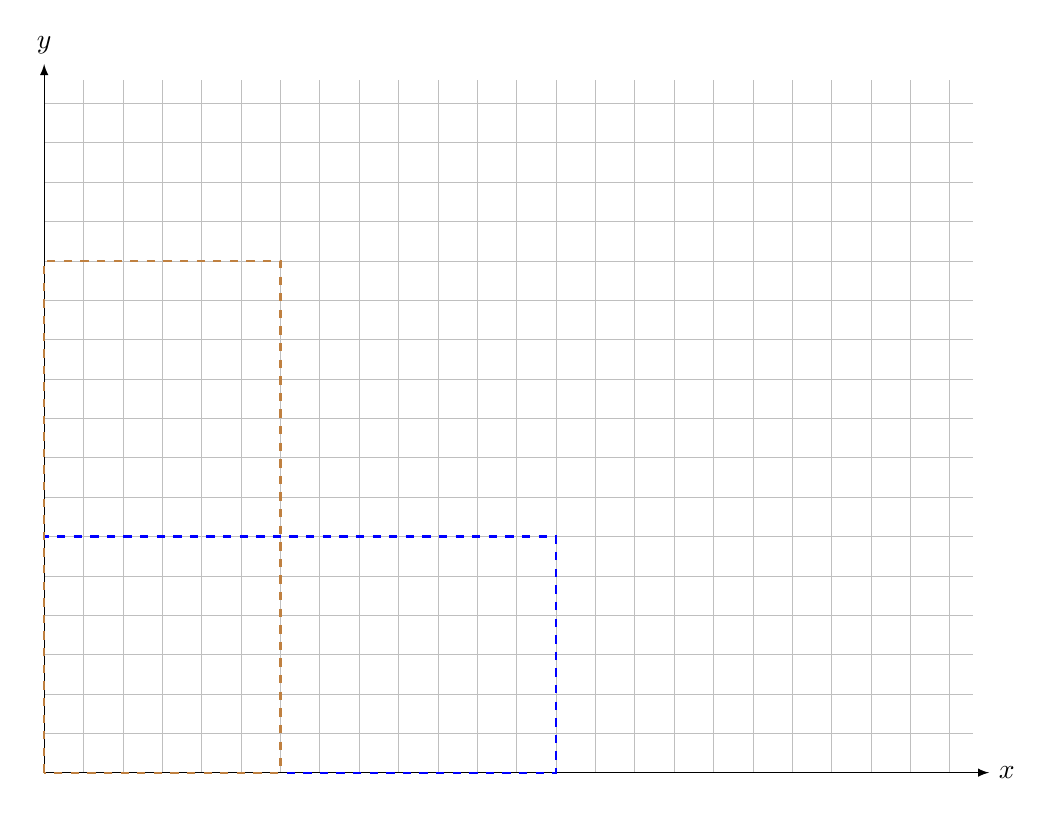
\begin{tikzpicture}
    \draw[step=.5cm,gray!50!white,very thin] (0,0) grid (11.8, 8.8);%(5.8,4.3);
    \draw[-latex] (0,0) -- (12,0) node [anchor=west] {$x$};
    \draw[-latex] (0,0) -- (0,9) node [anchor=south] {$y$};

    \draw[blue,thick,dashed] (0,0) rectangle (6.5,3);
    \draw[brown,thick,dashed] (0,0) rectangle (3,6.5);
  \end{tikzpicture}

  \caption{The rotation of the rectangle}\label{fig:rotofrect}
\end{figure}

\begin{figure}[h]\centering
 \includegraphics[width=0.9\textwidth]{xytrans-1.png}\\
 \includegraphics[width=0.9\textwidth]{xytrans-2.png}\\
 \caption{The rotation of the rectangle}\label{fig:rotofrect}
\end{figure}

Let's say that the origin state of one supertile:
The maximum length is $X_{max}$; The maximum width is $Y_{max}$; The related position of one tile of the supertils is $(x_0,y_0)$.
After $90^{\circ}$ of rotating, the position of the tile related to the new supertile will change to:
$X_{90^{\circ}} = y_0; Y_{90^{\circ}} = X_{max} - 1 - x_0;$
After $180^{\circ}$ of rotating, the position of the tile related to the new supertile will change to:
$X_{180^{\circ}} = X_{max} - 1 - x_0; Y_{180^{\circ}} = Y_{max} - 1 - y_0;$
And after $270^{\circ}$ of rotating, the position of the tile related to the new supertile will change to:
$X_{270^{\circ}} = Y_{max} - 1 - y_0; Y_{270^{\circ}} = x_0;$

 \item The overlapped range of two supertile

The program only need to check the overlapped range of two supertiles when apply the Mesh Testing.

Let's say two supertiles, $S_{test}$ and $S_{base}$, which are defined previously, will be tested. The maximum length of Base is MaxBaseX and the maximum wide of Base is MaxBaseY. The maximum length of Test is MaxTestX and the maximum wide of Test is MaxTestY. To avoid the negative value, the Base supertile is placed at (MaxTestX, MaxTestY). The Test can be placed (the top-left position $(x_0,y_0)$ of the Test rectangle) at any position at the range of ([0,MaxTestX+MaxBaseX), [0,MaxTestY+MaxBaseY)). See the figure.

Two basic conditions should be considered when calculate the overlap range. Let's consider the situation on the X axis. The two condition is that the length of the Test is less or large than that of Base.

%% Draw the length notation
%% #1-color, #2-text, #3-x, #4-y, #5-length
\newcommand*{\drawlennotation}[5]{%
    \draw[#1] (#3, 0.1 + #4) -- (#3, -.1 + #4);
    \draw[#1] (#3 + #5, 0.1 + #4) -- (#3 + #5, -.1 + #4);
    \draw[<->,#1] (#3,#4) -- (#3 + #5, #4);
    \draw[#1] (#3 + 0.5 * #5, #4) -- (#3 + 0.5 * #5, #4 + 0.1) node [anchor=south] {#2};
}

\begin{figure} \centering
  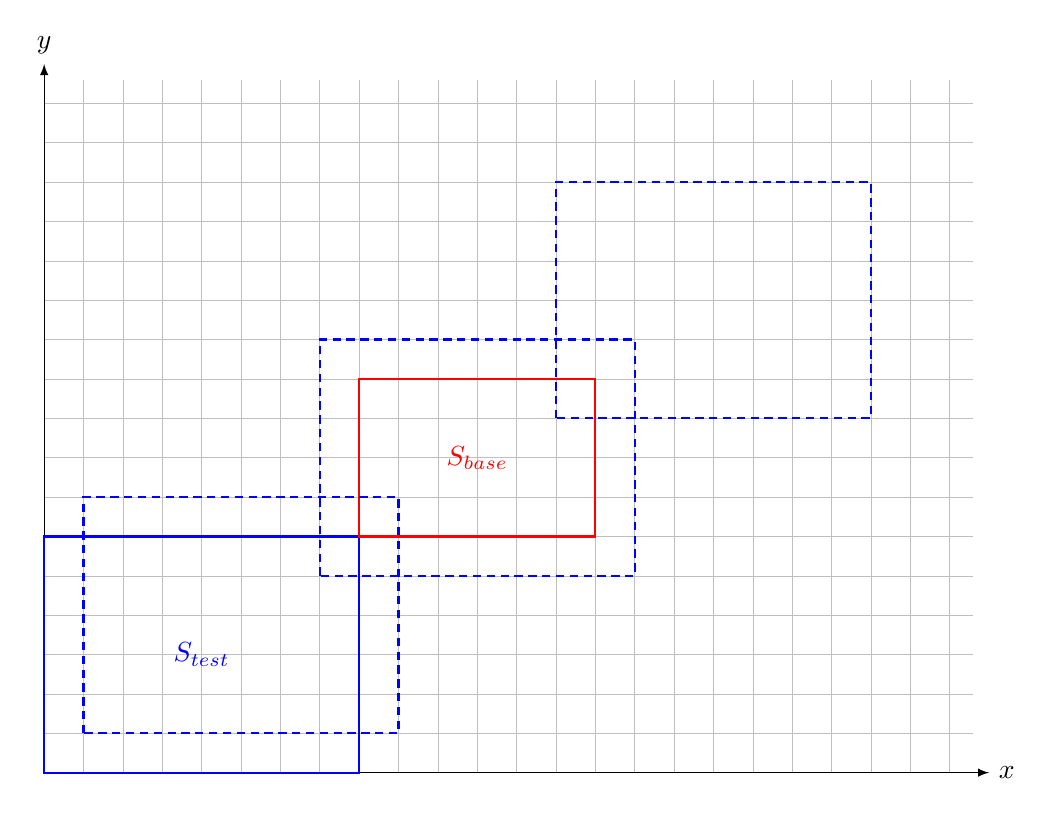
\begin{tikzpicture}
    \draw[step=.5cm,gray!50!white,very thin] (0,0) grid (11.8, 8.8);%(5.8,4.3);
    \draw[-latex] (0,0) -- (12,0) node [anchor=west] {$x$};
    \draw[-latex] (0,0) -- (0,9) node [anchor=south] {$y$};

    \draw[blue,thick] (0,0) rectangle (4,3) (2,1.5) node {$S_{test}$}; % 4,3
    \draw[red,thick] (4,3) rectangle (7,5) (5.5,4) node {$S_{base}$}; % 3,2

    \draw[blue,thick,densely dashed] (.5,.5) rectangle (4.5,3.5);
    \draw[blue,thick,densely dashed] (3.5,2.5) rectangle (7.5,5.5);
    \draw[blue,thick,densely dashed] (6.5,4.5) rectangle (10.5,7.5);

    \drawlennotation {blue} {MaxTest} {6.5}{7.75}{4}
    \drawlennotation {red} {MaxBase} {4}{5.75}{3}
  \end{tikzpicture}

  \caption{The overlap of the supertiles $S_{base}$ and $S_{test}$ (MaxBase $\leq$ MaxTest)} \label{fig:overlapsupertilele}
\end{figure}

\begin{figure} \centering
  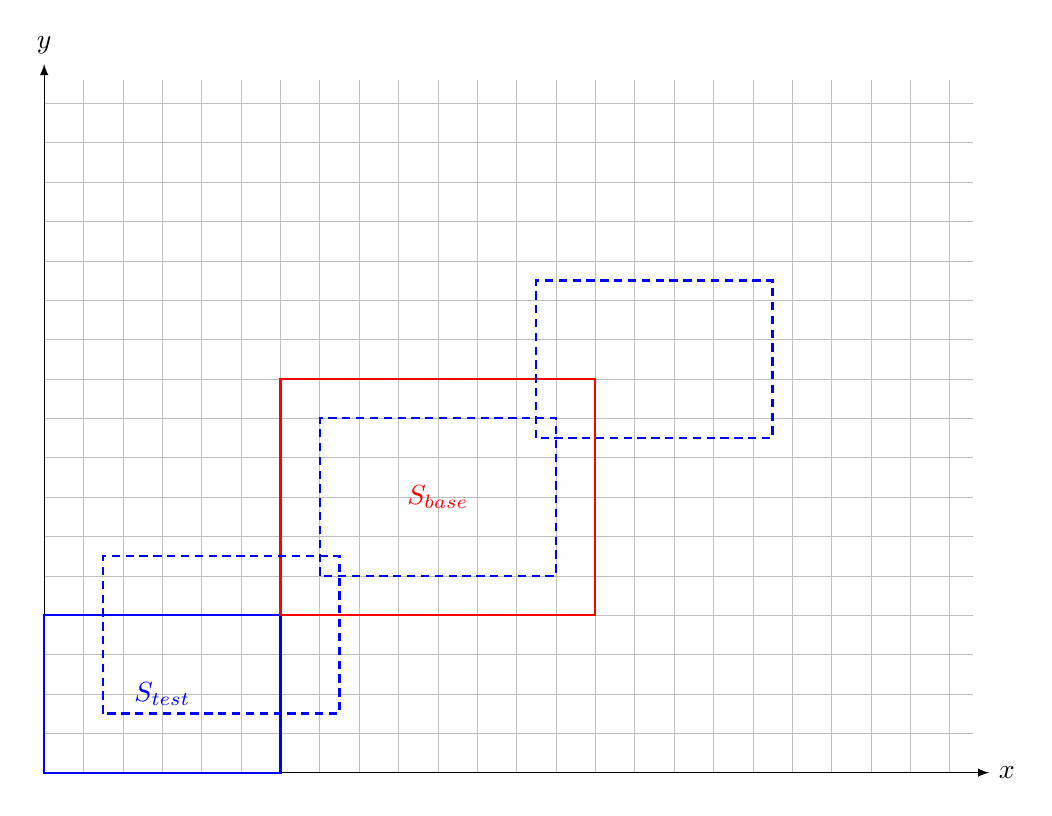
\begin{tikzpicture}
    \draw[step=.5cm,gray!50!white,very thin] (0,0) grid (11.8, 8.8);%(5.8,4.3);
    \draw[-latex] (0,0) -- (12,0) node [anchor=west] {$x$};
    \draw[-latex] (0,0) -- (0,9) node [anchor=south] {$y$};

    \draw[blue,thick] (0,0) rectangle (3,2) (1.5,1) node {$S_{test}$}; % 3,2
    \draw[red,thick] (3,2) rectangle (7,5) (5,3.5) node {$S_{base}$}; % 4,3

    \draw[blue,thick,densely dashed] (.75,.75) rectangle (3.75,2.75);
    \draw[blue,thick,densely dashed] (3.5,2.5) rectangle (6.5,4.5);
    \draw[blue,thick,densely dashed] (6.25,4.25) rectangle (9.25,6.25);

    %\drawlennotation {blue} {MaxTest} {6.5}{7.75}{4}
    %\drawlennotation {red} {MaxBase} {4}{5.75}{3}
  \end{tikzpicture}

  \caption{The overlap of the supertiles $S_{base}$ and $S_{test}$ (MaxBase > MaxTest)} \label{fig:overlapsupertilegt}
\end{figure}

\begin{table}\caption{The Absolute Position of the Overlaped Area ($PX_{abs}$)}
 \begin{tabular}{|r|l|l|}
 \hline
&{\bf Range of $x_0$}  &{\bf Absolute Position($PX_{abs}$)}\\
 \hline
                                 &[0, MaxBaseX)&[MaxTestX, MaxTestX + $x_0$)\\
 $Len_{Test} \textless Len_{Base}$&[MaxBaseX, MaxTestX)&[MaxTestX,MaxTestX+MaxBaseX)\\
                                 &[MaxTestX, MaxTestX + MaxBaseX)&[$x_0$, MaxTestX + MaxBaseX)\\
 \hline
                                     &[0, MaxTestX)&[MaxTestX, MaxTestX + $x_0$)\\
 $Len_{Test} \textgreater Len_{Base}$&[MaxTestX, MaxBaseX)&[$x_0$, MaxTestX + $x_0$)\\
                                     &[MaxBaseX, MaxTestX + MaxBaseX)&[$x_0$, MaxTestX + MaxBaseX)\\
 \hline
 \hline
                                     &{\bf Range of $y_0$}&{\bf Absolute Position ($PY_{abs}$)}\\
 \hline
                                     &[0, MaxBaseY)&[MaxTestY, MaxTestY + $y_0$)\\
$Width_{Test} \textless Width_{Base}$&[MaxBaseY, MaxTestY)&[MaxTestY,MaxTestY+MaxBaseY)\\
                                       &[MaxTestY, MaxTestY + MaxBaseY)&[$y_0$, MaxTestY + MaxBaseY)\\
 \hline
                                        &[0, MaxTestY)&[MaxTestY, MaxTestY + $y_0$)\\
$Width_{Test} \textgreater Width_{Base}$&[MaxTestY, MaxBaseY)&[$y_0$, MaxTestY + $y_0$)\\
                                        &[MaxBaseY,MaxTestY + MaxBaseY)&[$y_0$, MaxTestY + MaxBaseY)\\
 \hline
\end{tabular}
\end{table}

We can use the following formula to calculate the position of  the point related to each supertile:\\
Test: $P_{abs} - x_0$\\
Base: $P_{abs} - MaxTest$

So we use the absolute position to denote the position of the tiles.

 \item Plumb Testing
The Plumb Testing(PT) is the core algorithm of the system. We can use this algorithm to find out all of the position that two supertiles can mesh with. The algorithm could be described by the Algorithm \ref{alg:plumbtest}.

\begin{algorithm}
\caption{Plumb Testing} \label{alg:plumbtest}
\linesnumberedhidden
%\SetKwData{encset}{$\mathcal{E}$}
%\SetKwData{strengthset}{$S_{2d,2t}$}
%\SetKwData{tilein}{$T_{2d,2t}$}

\KwIn{$(x_0,y_0)$, the start position\\
$S_{base}$, the base supertile\\
$S_{test}$, the test supertile\\
$\tau$, the temperature of the system\\
$BG_{pos}$, the positions which are already visited
}

\KwOut{$L_{pos}$, the set of postions which are suitable to combine two supertiles}
    $L_{pos} \gets \phi $ \;
    $STK_{pos} \gets (x_0,y_0) $ \tcc*[r]{Push the start position to position stack}

    \While {$STK_{pos} \neq \phi $} {
        Pop one item from the top of stack $STK_{pos}$ to $(x,y)$ \;
        \If {$(x,y) \notin BG_{pos}$} {
            \tcc {It's not test at position $(x,y)$}
            $BL_{pos} \gets \phi $ \tcc*[r] {The positions which are pushed to stack}
            Get the overlap region of the two supertiles, $S_{base}$ and $S_{test}$ \;
            cnt[north] $\gets$ 0; cnt[east] $\gets$ 0; cnt[south] $\gets$ 0; cnt[west] $\gets$ 0 \;
            \tcc{Check each tile of the supertile $S_{test}$ in the overlap region}
            \For {each tile $t_0$ of $S_{test}$ in overlap region} {
                strength $\gets 0$ \;
                \For {each side of $t_0$ $s \in \{$north,east,south,east$\}$} {
                    \If {exist tile $t_1$ of $S_{base}$ near the side $s$ of $t_0$} {
                        \If {the glue type of $t_1$ at the side opposite($s$) is the same of glue $t_0$ at side $s$ } {
                            strength $\gets$ strength + glue strength \;
                            \tcc {Add 1 to the tile number of $S_{base}$ which is abut with the  tile of $S_{test}$ in this direction}
                            cnt[$s$] $\gets$ cnt[$s$] + 1 \;
                        }
                    }
                }
            }
            \If {strength $\geq \tau$} {
                $L_{pos} \gets L_{pos} \cup \{(x,y)\}$ \;
            }
            \For {each $s \in \{$ north,east,south,east $\}$} {
                $(x_2,y_2)$ is the position at the side of $t_0$ \;
                \If {cnt(s)=0 and $(x_2,y_2) \notin BG_{pos}$ and $(x_2,y_2) \notin BL_{pos}$} {
                    \tcc{there are no tiles of Base, the Test supertile can be moved to this direction to detect the mesh}
                    Push the position at the side of $t_0$ to stack $STK_{pos}$ \;
                    \tcc {Set the position $(x_2,y_2)$ as local accessed}
                    $BL_{pos} \gets BL_{pos} + \{(x_2,y_2)\}$ \;
                }
            }
            \tcc{Set the position $(x,y)$ as accessed}
            $BG_{pos} \gets BG_{pos} + \{(x,y)\}$ \;
        }
    }
    \KwRet{$L_{pos}$}\;
\end{algorithm}

 \item \bf{Split Algorithm}
In order to support the multi-stage (temperature) simulation, the split of the supertile should be processing

\end{enumerate}

\end{enumerate}

\section{The Algorithms of 3D Simulation}
The differences between the 2D and 3D simulations:
\begin{enumerate}
  \item The status of position of one tile cube.
  \item the rotations of the tile cube.
  \item 
\end{enumerate}

\end{document}